%\include{macro_lecture}
\section*{Cíl laboratorního cvičení}
\begin{itemize}
  \item seznámit se s nástroji pro správu sítě
  \item naučit se práci s nástrojem SSH a správu klíčů 
  \item naučit se pracovat s protokolem Syslog a nástrojem rsyslog
  \item konfiguraci nástrojů pro monitoring Icinga2
\end{itemize}

\section*{Pokyny}
\begin{itemize}
  \item Do zadání nepište, slouží pro další skupiny. PDF verzi zadání
  i šablony konfiguračních souborů lze najít v IS u předmětu ISA.
  
  \item Na konci laboratorního cvičení nezapomeňte na poslední bod,
  tj. na {\bf Ukončení práce v laboratoři}!
  
  \item Zapnete si počítače pod Windows prihlaste se jako užívatel \textbf{root} s heslem \textbf{root4lab}
  \item Zapnete si VirtualBox kde se nacházejí 3 virtuální počítače. Zkontrolujte zda jsou všechny počítače v předdefinovaném stavu init.
  
  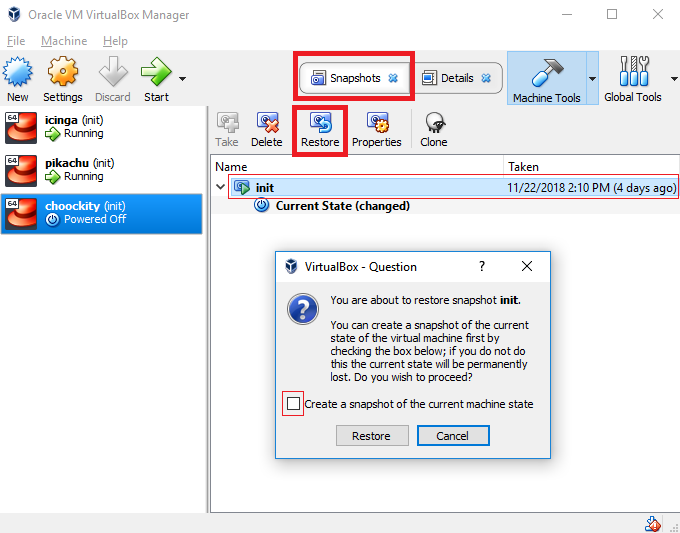
\includegraphics[width=\linewidth]{files/init.PNG}
  \item Všechny virtuální počítače mají 2 účty zapsané ve formě \textit{login/password}:
            \begin{itemize}
                \item \textbf{user/user4lab}
                \item \textbf{root/root4lab}
            \end{itemize}
\end{itemize}

\newpage
%\section{Laboratorní úlohy}
\section{Vzdálený terminál -- SSH}

Pracujte pod virtuálním počítačem pikachu a uživatelem {\tt user}. Zkontrolujte, že pracujete pod
uživatelem {\tt user} příkazem {\tt whoami}, který vypisuje jméno aktivního
uživatele.

Namísto řetězce {\tt <login>} používejte své studentské přihlašovací jméno.

\begin{enumerate}

  \item Pod uživatelem root ukončete démona spravujícího hesla k použitým klíčům SSH: 
  \begin{lstlisting}
  [user@pikachu]# su
  [root@pikachu]# pkill ssh-agent
  [root@pikachu]# exit
  \end{lstlisting}

  \item {\bf Bezpečné připojení na vzdálený počítač bez autentizačních klíčů.}

    \begin{enumerate}

      \item Přihlaste se příkazem {\tt ssh user@icinga} a zadejte heslo \textbf{user4lab}.

      \item Příkazem {\tt exit} nebo stiskem {\tt Ctrl-D} spojení ukončete.

    \end{enumerate}

  \item {\bf Vytvoření veřejného a privátního klíče.}

    \begin{enumerate}

      \item Příkazem {\tt ssh-keygen} vygenerujte implicitní klíč. Neměňte jeho
        název a zvolte heslo o délce alespoň osmi znaků například \textbf{pikapika}.

      \item Příkazem \verb|ssh-keygen -N "" -f ~/.ssh/nopass -C <login>@nopass| vygenerujte autentizační klíč bez hesla.

      \item Příkazem {\tt ssh-keygen -N <heslo> -f \textasciitilde/.ssh/pass -C
        <login>@pass} vygeneruje klíč s heslem jiným než pro výchozí klíč například \textbf{12345678}.

      \item Ověřte obsah a přístupová práva u nově vzniklých souborů (ls -l \textasciitilde/.ssh). Jak
se liší práva mezi souborem s privátním a veřejným klíčem?

    \end{enumerate}

  \item {\bf Distribuce klíčů}

    \begin{enumerate}

      \item Všechny tři veřejné klíče si zkopírujte na vzdálený počítač do
        souboru \verb|.ssh/authorized_keys|.
        (např. {\verb&ssh-copy-id -i <cesta k veřejnému klíči> <user>@<server>&}).
        
      Jaké heslo bylo nutné zadat?

      \item Zkuste se znovu přihlásit na stejný vzdálený počítač. Jaké heslo bylo nyní nutné zadat? Zkuste
zadat špatné heslo a pozorujte, které další klíče se použily. Při experimentech můžete také
využít tzv. verbose režim ssh ({\tt ssh -v}). Pro experimenty s identitou
využijte přepínač~{\tt -i}.

    \end{enumerate}

  \item {\bf Konfigurace použití klíčů}

    \begin{enumerate}

      \item Stejným způsobem nakopírujte své veřejné klíče ještě na další počítač \textbf{choockity}.

      \item Na svém počítači vytvořte soubor \textbf{\textasciitilde/.ssh/config} a pomocí textového editoru přidejte
        nasledující konfiguraci (hostname definujte jen pro jeden ze dvou strojů, na který jste
        kopírovali veřejné klíče):
        \begin{verbatim}
            Host icinga
                IdentityFile ~/.ssh/id_rsa

            Host *
                IdentityFile ~/.ssh/pass
                IdentityFile ~/.ssh/nopass
        \end{verbatim}
    \item Zmente prava v subore \textit{~/.ssh/config} pomoci príkazu:
      \begin{lstlisting}
        [user@pikachu]# chmod 600 ~/.ssh/config
      \end{lstlisting}
    
    \item Přihlaste se postupně na oba počítače. Které klíče se použily? Co se stane, když
pro některý klíč zadáte špatné heslo?

    \end{enumerate}

  \item {\bf Omezení použití klíčů}

    Nyní bude naším cílem omezit použití klíče, který není chráněn heslem tak,
    aby pomocí něj bylo možné na vzdáleném serveru vykonat pouze konkrétní příkaz.

    \begin{enumerate}

      \item Přihlaste se na počítač, kam jste nakopírovali své veřejné klíče a
        upravte soubor s autorizovanými veřejnými klíči tak, že na začátek
        řádku s klíčem nopass (řádek poznáte tak, že končí řetězcem
        {\tt <login>@nopass}) napíšete
        \verb|command="cat /etc/passwd" | (od původního
        obsahu oddělený jednou mezerou).

      \item Odhlaste se ze vzdáleného počítače icinga a znovu se na něj přihlaste
        příkazem {\tt ssh icinga -i \textasciitilde/.ssh/nopass}. Aplikovalo se
        omezené využití klíče?

    \end{enumerate}


  \item {\bf Pohodlné opakované použití klíče zabezpečeného heslem.}

    \begin{enumerate}

      \item Spusťte program ssh-agent:
      \begin{lstlisting}[language=bash]
            [user@pikachu]# eval $(ssh-agent -s)
      \end{lstlisting}

      \item Přidejte váš vygenerovaný klíč pomocí příkazu a zadejte heslo:
        \begin{lstlisting}[language=bash]
            [user@pikachu]# ssh-add ~/.ssh/id_rsa
            Enter passphrase for .ssh/id_rsa:
        \end{lstlisting}
      \item Přihlaste se k serveru icinga. Museli jste zadávat znovu heslo?
    \end{enumerate}
  \item Ověření konfigurace
    \begin{enumerate}
        \item Přihlaste se na počítač icinga (malo by to jet bez hesla)
        \item Použijte příkaz \textbf{ssh-add -d} a následně se opět přihlaste na 
        počítač icinga a stisknete 3 krát enter (měl by se vypsat obsah souboru /etc/passwd)
        \item Přihlaste se na počítač choockity a zadaje heslo 12345678
        \item Přihlaste se opět na počítač chockity, stisknete 2 krát enter.
    \end{enumerate}
  \item Pokud vám vše správně fungovalo vypnete počítač choockity, nebudeme ho v následujících úkolech potřebovat.

\end{enumerate}


\section{Syslog}
  \begin{itemize}
    \item Úkol: 
    \begin{itemize}
      \item Seznámit se s protokolem Syslog, který slouží pro přenos
      logovacích zpráv ze spravovaných zařízení. Pojmem Syslog je často označováno také
      programové vybavení implementující samotný přenos, třídění a ukládání zpráv na disk.
      \item Stanici \textbf{pikachu} si zvolte jako klient a \textbf{icinga} jako server a 
      nakonfigurujte přeposílání veškerých Syslog zpráv z klienta na server. Mějte na paměti 
      možné zneužití Syslog protokolu útočníkem a omezte na straně serveru příjem pouze na 
      zprávy od daného klienta a klientovi zamezte příjem jakýchkoliv zpráv ze sítě.
      \item Pro práci využijte nástroj {\tt rsyslogd}, který bude sloužit jako server i klient.
      K otestování využijte nástroj {\tt logger}.
      \item Na klientovi následně omezte přeposílání pouze na zprávy konkrétního typu.
      \item Na obou stanicích pracujte jako uživatel root.
    \end{itemize}
    \item Příkazy:
       \begin{itemize}
            \item {\tt rsyslogd(8)} -- démon pro Syslog.
            \item {\tt rsyslog.conf(5)} -- Popis konfigurace rsyslog démona.
            \item {\tt logger(1)} -- Nástroj pro generování Syslog zpráv.
            \item {\tt tcpdump(1)}
        \end{itemize}
    \item Postup:
       \begin{enumerate}
            \item {\bf Na serveru} povolte naslouchání na síťovém soketu. Do souboru {\tt /etc/rsyslog.conf} přidejte nebo odkomentujte:
\begin{verbatim}
  $ModLoad imudp
  $UDPServerRun 514
\end{verbatim}

            \item {\bf Na klientovi} zakažte programu rsyslogd naslouchat na síťovém soketu,
tj. odeberte/zakomentujte v souboru {\tt /etc/rsyslog.conf} řádky:
\begin{verbatim}
  $ModLoad imudp
  $UDPServerRun 514

  $ModLoad imtcp
  $InputTCPServerRun 514
\end{verbatim} 

            \item {\bf Na klientovi} nakonfigurujte rsyslog démona tak, aby odesílal veškeré zprávy
         z klienta na serveri pomocí UDP. Jako oddělovač použijte výhradně tabulátor nikoliv mezery.
         Do souboru {\tt /etc/rsyslog.conf} přidejte následující pravidlo:
\begin{verbatim} 
 *.*<TAB>@<doménové_jméno_serveru>:<číslo_portu>
\end{verbatim}

            \item {\bf Na serveru i klientovi} restartujte Syslog démona: 
\begin{verbatim}
  systemctl restart rsyslog
\end{verbatim} 

            \item {\bf Z klienta} ověřte správnou konfiguraci vygenerováním testovací Syslog 
         zprávy pomocí nástroje {\tt logger}:
\begin{verbatim} 
  logger -d <obsah_zprávy>
\end{verbatim} 
        
            \item Zpráva byla přeposlána na server, kde ji lze najít na konci souboru
         {\tt /var/log/messages}.

\begin{verbatim} 
  tail -f /var/log/messages | grep <doménové_jméno_klienta>
\end{verbatim} 

            \item  Na klientovi pokračujte v generování Syslog zpráv a 
         na serveru sledujte příchozí Syslog zprávy pomocí {\tt tcpdump}. Na jakém
         portu a jakým protokolem jsou Syslog zprávy zasílány.
         
         

            \item Otevřete si manuálovou stránku rsyslog.conf a zjistěte, jaké zařízení a priority
         zpráv Syslog poskytuje. FIXME konkretizovat
\begin{verbatim} 
  man rsyslog.conf
\end{verbatim} 
        
         \item Ze znalosti zařízení a priorit nakonfigurujte klienta, aby posílal na server 
         pouze zprávy při selhání autentizace, tj. upravte již existující pravidlo pro přeposílání
         veškerých zpráv na server v souboru {\tt /etc/rsyslog.conf}. Nezapomeňte restartovat Syslog démona. 
         
\begin{verbatim} 
  Syntax pravidel: <facility>.<priority><TAB><action>
\end{verbatim} 
         \item Ze serveru se následně pokuste o neúspěšné ssh připojení na klienta a podívejte se
         do souboru pro autentizační záznamy, jakou zprávu zaslal klient serveru.


       \end{enumerate}
   \end{itemize}

\section{Icinga2}
  \begin{itemize}
    \item Úkol: 
    \begin{itemize}
      \item Seznámit se s nástrojem Icinga2 pro monitorováni zařízení a servisů 
      \item Na klientské stanici nakonfigurovat nakonfigurovat kontroly servisů a hostů.  
    \end{itemize}
    \item Poznámka:
        \begin{itemize}
            \item Na počítačích icinga a pikachu pracujeme pod uživatelem \textbf{root}
        \end{itemize}
    \item Postup:
       \begin{enumerate}   
            \item Ve Windows si otevřete webový prohlížeč a zadejte adresu 
            \textit{http://10.0.2.3}. Dostanete se na webové rozhraní Icingy2,
            která běží na počítači \textbf{icinga}.
               \begin{enumerate}
                   \item Přihlaste se pod uživatelem \textbf{user} a heslem \textbf{user4lab}
                    \item Přesměruje Vás to na rozhraní kde si můžete všimnout monitoring odledně localhost zařízení.
               \end{enumerate}
            \item Na zařízení icinga ve složce \textit{/etc/icinga2/conf.d} otevřete soubor \textbf{hosts.conf}, kde se nachází zakomentovaný příklad a do něj doplňte následující konfiguraci:
\begin{verbatim}
object Host "Pikachu" {
    address = "<IP ADDRESS>"
    check_command = "hostalive"
}

object Service "http" {
    max_check_attempts = 4
    check_interval = 10m
    retry_interval = 10m
    host_name = "<HOST NAME OF OBJECT>"
    check_command = "http"
}

\end{verbatim} 
            \item Restartujte službu
\begin{verbatim}
  systemctl restart icinga2.service
\end{verbatim} 
          \item Podívejte se na webové rozhraní Icingy2. Co se tam změnilo ? 
          Když je nějaká služba down proč tomu tak je ?

          \item Na klientském počítací jménem pikachu zapnete webový server
\begin{verbatim}
  python -m SimpleHTTPServer <port>
\end{verbatim}
          \item Ve Webovém rozhraní Icingy2 v menu Overview|Services si vyhledejte předešlí check na http službu. Pokud je služba down stisknete na odkaz \textit{Check Now}. Změnilo se něco oproti předešlému stavu z bodu 4?

          \item Jaký je interval mezi jednotlivými kontrolami pro Host Pikachu? Porovnejte tento interval s přednastaveními kontrolami. Jsou tyto intervaly rozdílné ? Pokud ano proč.

\end{enumerate}
\end{itemize}

\section*{Ukončení práce v laboratoři}
\begin{itemize}
  \item Vypnout všechny virtuální instance s odkliknu-tou možnosti obnovit na původní snímku init.
          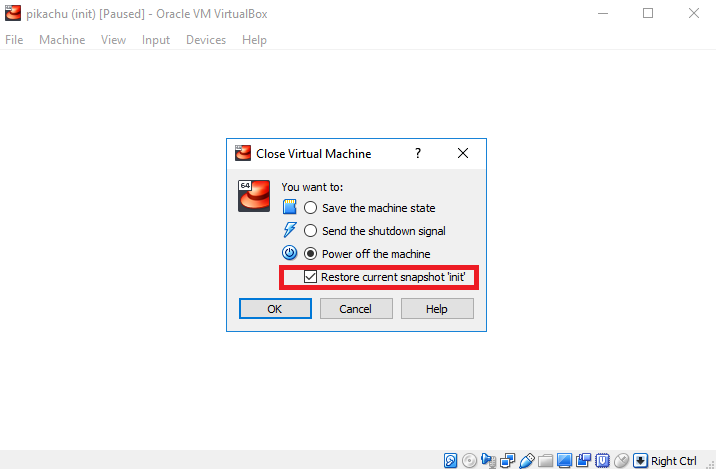
\includegraphics[width=\linewidth]{files/end.PNG}

\end{itemize}
